\chapter{ПРОЕКТИРОВАНИЕ \\ДВИГАТЕЛЬНОЙ УСТАНОВКИ}
ДУ образца представляет собой стартовый РДТТ на смесевом топливе.

Определение конструктивных параметров РДТТ будет осуществляться по результатам варьирования давления внутри камеры сгорания. Назначим следующий диапазон варьирования:
\[ \text{от 5 МПа до 25 Мпа, с шагом 1 МПа.}
\]

\paragraph{Исходные данные}

%\begin{table}[!h]
%	\begin{center}
%		\begin{tabular}{l l l}
%Калибр:				 &  & $D_\text{н}$=125 мм \\ 
%Полный импульс:		 &	& $J_\text{p}$= 3300 Н$\cdot$с \\ 
%Материал корпуса ДУ: &	& сплав СП-33 \\
%Время работы ДУ:	 &	& 3.5 с \\ 
%%					 &	$\rho_\text{м}$=7830  кг/м^3  \\ 
%%					 &	$\sigma_\text{вр}$=1650 Мпа	 \\ 
%%					 &	$\sigma_\text{02}$=1350 Мпа	 \\ 
%		\end{tabular}
%		\label{tab:hellfire_stats}
%	\end{center}
%\end{table}



\begin{enumerate}[1.]
	\item Калибр:				     $D_\text{н}$=125 мм  
	\item Полный импульс:		 	 $J_\text{p}$= 3300 Н$\cdot$с  
	\item Время работы ДУ:	 	3.5 с  
	\item Материал корпуса ДУ:
	\begin{enumerate}
 		\item сплав СП-33 
		\item $\rho_\text{м}$=7830  $\text{кг/м}^3$
		\item $\sigma_\text{вр}$=1650 МПа	  
		\item $\sigma_\text{02}$=1350 МПа	  
	\end{enumerate}
	\item Характеристики топлива: смесевое на основе традиционных компонентов \\
		Массовые доли и плотности компонентов топлива:
	\begin{enumerate}
		\item Синтетический каучук полибутадиеновый (\text{HTPB})	
			\begin{itemize}
				\item $g_1=0,14$		
				\item $\delta_1=920 \text{кг/м}^3$ 
			\end{itemize}
		\item Перхлорат аммония (ПХА)	
			\begin{itemize}
				\item $g_2=0,68$		
				\item $\delta_2=1950 \text{кг/м}^3$ 
			\end{itemize}
		\item Алюминий (Al)			
			\begin{itemize}
				\item $g_3=0,18$		
				\item $\delta_3=2700 \text{кг/м}^3$ 
			\end{itemize}
	\end{enumerate}
	\item Постоянные в законе скорости горения:
	\begin{itemize}
		\item $p_{ref}=5 $ МПа;
		\item $u_{ref} = 6,6$ мм/с;
		\item $\eta=0,23$
	\end{itemize}
	\item Зависимость от температуры $D_t=0,003 $ 1/(\textdegree C)
\end{enumerate}

\paragraph{Термодинамический расчёт энергетических характеристик ТРТ}

Условные химические формулы и энтальпии образования компонентов:
\begin{enumerate}[1.]
	\item HTPB: 			 $C_{70.75}H1_{06.5}O_{2.23}N_{0.63}	\Delta Hf_{298}=-580 $ кДж/кг;
	\item Перхлорат аммония: $  NH_4ClO_4	 		\Delta Hf_{298}=-2520 $ кДж/кг;
	\item Алюминий: 		 $ Al				\Delta Hf_{298}= 0 $ кДж/кг.
\end{enumerate}

Энтальпия образования топлива:
\begin{multline*}
	\Delta Hf_{298}=  C(\text{HTPB}) \cdot \Delta Hf_{298}(\text{HTPB}) + \\ + C(\text{ПХА}) \cdot \Delta Hf_{298}(\text{ПХА}) + \dots + C(Al) \cdot \Delta Hf_{298}(Al) = \\ = 0.14 \cdot (-580) + 0.68 \cdot (-2520) + \dots 	+ 0.18 \cdot (0) = -1795  \text{кДж/кг}
\end{multline*}

% Брутто-формула рабочего тела: $C_{9.89}H_{38.04}O_{23.46}N_{5.88}C_{l5.79}A_{l6.67}$

Термодинамические свойства продуктов сгорания:
\begin{enumerate}[1.]
	\item Температура продуктов сгорания (КС): 	$T_0 = 3367,5$ K;
	\item Уд. теплоёмкость при пост. давлении (КР): 	$c_p = 1,9105 \text{ кДж/кг} \cdot \text{К} $;
	\item Показатель адиабаты (КР): 				$k = 1,1511$;
	\item Газовая постоянная газовой фазы (КР):		$R_\text{г} = 436,52 \text{ кДж/кг} \cdot \text{К}$;
	\item Массовая доля конденсированной фазы (КР):		$Z = 0,32038$;
	\item Расходный комплекс:					$\beta = 160,03 $ с.
\end{enumerate}

Параметры адиабатического расширения до $p_a = 0,1$ МПа:

при равновесном расширении:
\begin{enumerate}[1.]
	\item Относительная площадь выходного сечения:	$F_\text{отн} = 6,9546$;
	\item Пустотный удельный импульс:				$I_\text{удп} = 277,40с$;
	\item Единичный импульс топлива:
$$I_{(40/1)}=(I_\text{удп}-\frac{p_\text{a}}{p} \cdot \beta \cdot F_\text{отн} ) \cdot g=(277,4-\frac{0,1}{4} \cdot 160,03 \cdot 6,9546) \cdot 9,81=2448,34 \text{ м/с;}$$
\end{enumerate}

при «замороженном» расширении:
\begin{enumerate}[1.]
	\item Относительная площадь выходного сечения:	$F_\text{отн} = 6,4957$;
	\item Пустотный удельный импульс:				$I_\text{удп} = 272,50$ с;
	\item Единичный импульс топлива:	
$$I_(40/1)=(I_\text{удп}-\frac{p_\text{a}}{p} \cdot \beta \cdot F_\text{отн} ) \cdot g=(272,50-\frac{0,1}{4} \cdot 160,03 \cdot 6,4957) \cdot 9,81=2418,29 \text{ м/с}$$
\end{enumerate}

\emph{Определение теплового эффекта реакции горения}

Камера сгорания:

\begin{figure}[!h]
\begin{center}
    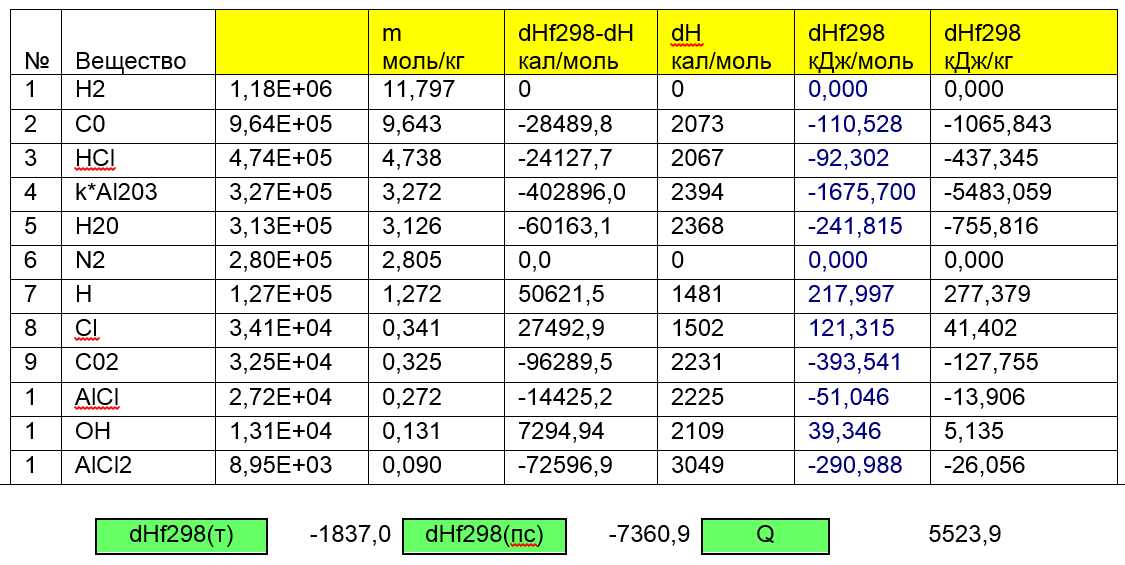
\includegraphics[width=1\linewidth]{appendix_table1.PNG}
    \label{fig:appendix_table1}
\end{center}
\end{figure}

\clearpage
Критическое сечение
\begin{figure}[!h]
\begin{center}
    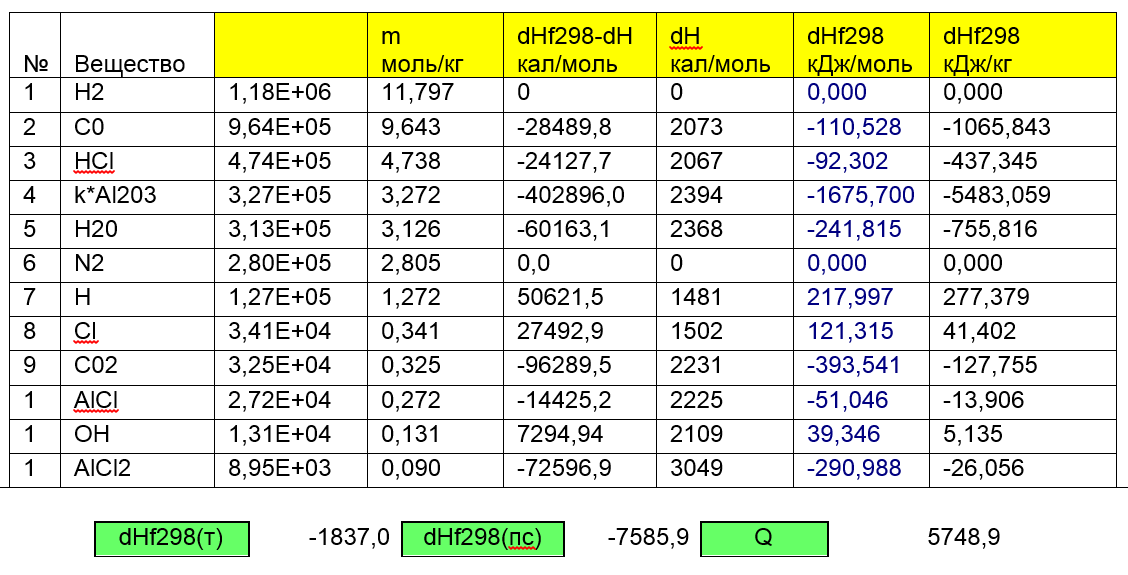
\includegraphics[width=1\linewidth]{appendix_table2.PNG}
    \label{fig:appendix_table2}
\end{center}
\end{figure}

Выходное сечение
\begin{figure}[!h]
\begin{center}
    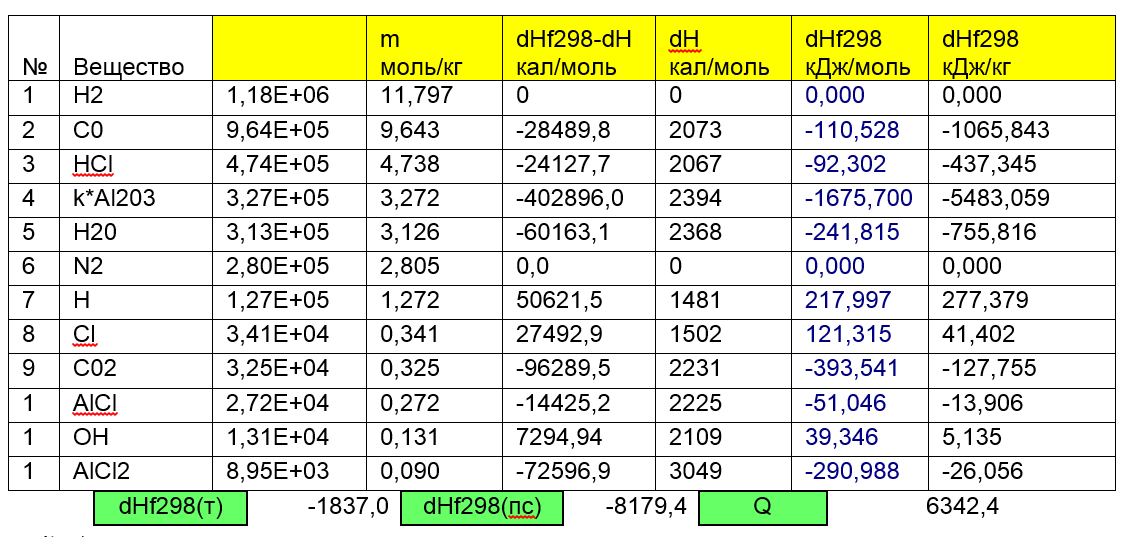
\includegraphics[width=1\linewidth]{appendix_table3.PNG}
    \label{fig:appendix_table3}
\end{center}
\end{figure}

\paragraph{Расчёт геометрических параметров заряда РДТТ}

\emph{Исходные данные для геометрического расчета:}
\begin{itemize}
	\item форма заряда:					звездообразная;
	\item наружный диаметр: 				$D_\text{н}=125$ мм;
	\item внутренний диаметр:				$D_\text{вн}=0,94 \cdot D_\text{н}=117$ мм;
	\item полный импульс:					$J_p=3300 \text{ Н} \cdot \text{с} $;
	\item единичный импульс топлива:		$J_\text{40/1}=2424,29$ (Н$\cdot$с)/кг;
	\item требуемая масса топлива:          $\omega = I_p/I_\text{40/1}$  = 1,36 кг.
\end{itemize}
Массовые доли и плотности компонентов топлива:
\begin{enumerate}
	\item Синтетический каучук полибутадиеновый (\text{HTPB})	
		\begin{itemize}
			\item $g_1=0,14$		
			\item $\delta_1=920 \text{кг/м}^3$ 
		\end{itemize}
	\item Перхлорат аммония (ПХА)	
		\begin{itemize}
			\item $g_2=0,68$		
			\item $\delta_2=1950 \text{кг/м}^3$ 
		\end{itemize}
	\item Алюминий (Al)			
		\begin{itemize}
			\item $g_3=0,18$		
			\item $\delta_3=2700 \text{кг/м}^3$ 
		\end{itemize}
\end{enumerate}

Плотность топлива:				$\delta = \frac{1} {\sum_i{\dfrac{g_i}{\delta_i}}}	 $ = 1761,9   кг/$\text{м}^3$. 

Требования к характеристикам заряда:
\begin{itemize}
	\item коэффициент заполнения:					$\epsilon \approx 0,75..0,9$ ;
	\item параметр Победоносцева:					$\kappa<150$ ;
	\item отклонение площади горения от среднего значения:	$\Delta S_\text{г}< \pm 5 $ \%.
\end{itemize}

\paragraph{Результаты расчета:}

Выбранные параметры заряда на стартовом участке:
\begin{itemize}
	\item толщина горящего свода:  				$е_1$ = 23 мм ;
	\item число лучей:						n = 7 ;
	\item угол раствора луча					33 \textdegree;
	\item радиус скругления луча 				3 мм.
\end{itemize}
									
\clearpage
Полученные характеристики заряда:
\begin{itemize}
	\item длина заряда :							L = 0,110 м ;
	\item средняя площадь поверхности горения:			$S_\text{ср} = 0,030 $ м2;
	\item коэффициент заполнения поперечного сечения ДУ:	$\epsilon= 0,77$ ;
	\item Процент содержания дегрессивных остатков: 		$\chi_\text{д} = 9,61$ \%;
	\item Максимальное отклонение от среднего значения:	$\Delta S_\text{ср}=4,95$ \%
\end{itemize}

\begin{figure}[!h]
\begin{center}
    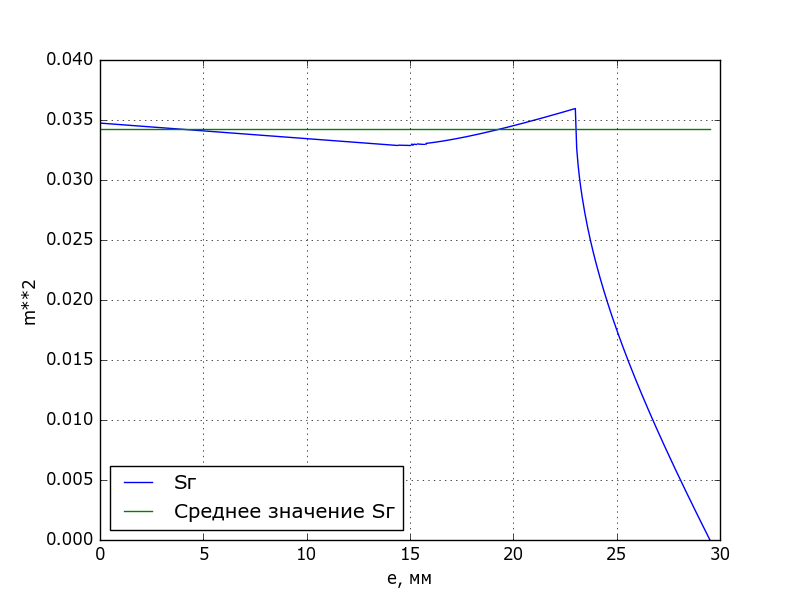
\includegraphics[width=1\linewidth]{appendix_sgor}
	\caption{Зависимость относительного изменения площади поверхности горения}
    \label{fig:appendix_sgor}
\end{center}
\end{figure}


\clearpage
\paragraph{Выбор проектных параметров ДУ минимальной массы}

\emph{Постоянные}

Характеристики ТЗП:
\begin{enumerate}
	\item Плотность 								$\rho_u=1500 $ кг/$\text{м}^3$
	\item Толщина								$\Delta _u=2.5$ мм
	\item Нормальная температура заряда				$t_N=18$ \textdegree
	\item Минимальная технологическая толщина стенки	$\Delta _{min}=1.5 $мм
	\item Постоянная коэффициента теплоотдачи			$\sigma_T=160$  (Вт$\cdot$м)/(кг$\cdot$К)
	\item Относительная разность температур газа и стенки	$\nu_T=0.7$
\end{enumerate}

\emph{Алгоритм расчета}

Задача решается путем варьирования давления в камере сгорания.
\begin{enumerate} 
	\item Диапазон варьирования давления: 					4 .. 16 МПа;
	\item Шаг варьирования:							1 МПа.
	\item В первом приближении принимаем $\omega = \omega_0$.
\end{enumerate}

\emph{Определение габаритов камеры сгорания}

Предварительные расчеты.
\begin{enumerate}
	\item Внутренний диаметр:				$D_\text{вн}=0.96 \cdot D_\text{н}$
	\item Площадь поперечного сечения:			$F_0=(\pi D_0^2)/4$
	\item Площадь горения:					$S=\omega/(e_1 \cdot \delta)$
	\item Влияние начальной температуры заряда:	$\phi(t_h)=e^{D_t (t_\text{н}-t_N)}$
	\item Влияние эрозионного горения:			$\phi(\kappa)=1+A(\kappa-\kappa_\text{пор} )$
	\item A = 0.003
	\item $\kappa_\text{пор}=100 $– пороговое значение параметра Победоносцева.
\end{enumerate}

\emph{Определение расчетного давления и потребной толщины стенки.}

Максимальное давление, реализуемое в камере сгорания:
$$p_{+50}=p \cdot \phi{+50}^{1/(1-\nu)}$$
Рабочее давление:
$$p_\text{р}=\sigma_\text{вр}/\sigma_{0,2}  K_\delta p \cdot K_\text{p} \cdot K_\eta \cdot p_{+50} \cdot \phi(\kappa)^{1/(1-\nu)}$$

$K_\delta p=1.1 $ – коэффициент, учитывающий всплеск давления при работе воспламенителя;

$K_p=1.2 $ – коэффициент, учитывающий разброс свойств топлива между партиями;

$K_\eta=1.25 $ – коэффициент запаса прочности;

$B_{H0}=  \sigma_\text{вр}/(\sigma_\text{вр}+p_p )$

Толщина стенки:			$\delta_0=D_H/2 (1-B_H0 )$;

Выбирается наибольшее значение из полученной толщины $\Delta_0$ и минимальной толщины, которая может быть получены технологически $\Delta _{min}$

$\Delta = max(\Delta_0; \Delta _{min})$

$B_H=1-2\Delta/D_H $

Внутренний диаметр обечайки:		$D=D_H  - 2\Delta $

$B_K=1-(2\Delta _u)/D$

Внутренний диаметр камеры:		$D_\text{ВH}=D - 2\Delta _u $

$F=(\pi D_\text{BH}^2)/4$

Длина заряда:				$L=(\omega \cdot (1+\xi_\text{д}))/(\delta \cdot F \cdot \epsilon)$


\paragraph{Расчет внутрибаллистических характеристик РДТТ}

\emph{Оценка газоприхода}
Скорость горения:				$u=u_1 \cdot p^\nu$

Газоприход:					$G_\text{п}=S \cdot u \cdot \Delta$;

\emph{Оценка потерь на теплоотдачу}
Площадь охлаждения:			$F_\text{охл}=K_L \cdot \pi  \cdot D_\text{ВH} \cdot L$

$K_L=1.04$  – коэффициент, учитывающий отношение длины обечайки к длине заряда.

Коэффициент тепловых потерь:	
$$	\chi_T=1-(\sigma_T \cdot \nu_T \cdot F_\text{охл} \cdot p)/(R \cdot Q \cdot ) G_\text{п}$$

Температура продуктов сгорания: 	$T=\chi_T \cdot T_0$

\emph{Определение размеров критического сечения}

$\rho=p/(R \cdot T)$

Расход через сопло:			$G_\text{р}=G_\text{п} \cdot (1-\rho/\Delta)$

Площадь критического сечения:	$F_\text{кр}=G_\text{р} \cdot \frac{\sqrt{R \cdot T}}{А_1 \cdot p}$
$$ A_1=\sqrt{k \cdot ( \dfrac{2}{k+1})^{\dfrac{k+1}{k-1} } }$$

Диаметр критического сечения:		$d_\text{кр}=\sqrt{(4 \cdot F_\text{кр})/\pi }$

\emph{Определение размеров выходного сечения}

Диаметр выходного сечения:		$D_\text{вых0}=K_\text{Dвых} \cdot D_H$
$K_\text{Dвых}=0.8$  – коэффициент, учитывающий отношение диаметров выходного сечения к внешнему.

Площадь выходного сечения:	$F_\text{вых0}=\pi /4 \cdot  D_\text{вых0}^2$

Проверка из условия не достижения перерасширенного сопла: 
$$q(\lambda )= \lambda  \cdot \left(\frac{1-(k-1)/(k+1) \cdot \lambda ^2}{2/(k+1)} \right) ^{\dfrac{1}{k-1}}$$

Находится значение $\lambda _\text{в1}$, удовлетворяющее условию: 
$$q(\lambda )=F_\text{кр}/F_\text{вых0} $$

Находится значение:  $\lambda _\text{в2}=\lambda _\infty \cdot \sqrt{1-p_a/p)} ^{\dfrac{k-1}{k}}$

Расчет ведётся по минимальному значению: $\lambda _\text{в} = min(\lambda _\text{в1}; \lambda _\text{в2})$

Уточняется значение площади выходного сечения:	
$$F_\text{вых}=F_\text{кр}/(q(\lambda _\text{в}))$$

\emph{Расчет тяги и удельного импульса РДТТ}

Теоретический коэффициент реактивности:	
		$$K_\text{втеор}=\frac{\lambda _\text{в}+ \lambda _\text{в}^{-1}}{2}$$

Действительный коэффициент реактивности:
$$K_\text{в}=\chi_\mu \cdot \left(1+\chi_\theta \cdot \chi_\text{н} \cdot (K_\text{втеор}-1) \right)$$

$\chi_\mu=0.98 $ – коэффициент, учитывающий потери от диссипации,

$\chi_\theta=0.95$ – коэффициент, учитывающий потери от неодномерности,

$\chi_\text{н}=1 $ – коэффициент, учитывающий потери от нестационарности;


Предельное значение удельного импульса:	$J_\infty=2 \sqrt{\cdot \chi_T \cdot Q_\text{ж} }$

Удельный импульс:				
$$	J_\text{уд}=J_\infty \cdot \frac{K_\text{в}}{K_\infty}  \cdot \chi_\text{кф}-\frac{F_\text{вых} \cdot p_a}{G_p} $$

$\chi_\text{кф} $ -  коэффициент учета потерь, связанных с многофазностью продуктов сгорания

$$\chi_\text{кф}=\dfrac {1+\xi \cdot K_\nu \cdot \dfrac{\lambda _\text{в}}{\lambda _\infty}  \cdot \dfrac{K_\infty}{K_\text{в}} }  {\sqrt{(1+\xi) \cdot (1+\xi \cdot \overline{c_p} ) }},$$
 где $K_\nu=0.9$ и $\overline{c_p}=0.8 $

Требуемая масса топлива:		$\omega `= \frac{J_p}{J_\text{уд}} $

Если условие $|1- \frac{\omega'}{\omega}| \le 0.1$ \% не выполняется, то в качестве $\omega_0$
назначается  $\omega`$ и расчеты повторяются до тех пор, пока не будет выполняться данное условие. 

\paragraph{Расчет воспламенителя}

Геометрические параметры заряда на данном этапе известны. Согласно [???], массу воспламенителя можно определить по следующей эмпирической формуле:
$$m_\text{в}=q \cdot S_\Sigma/Q_\text{в} $$
Здесь q = 30 Дж/см2 – количество тепла, необходимое для воспламенения единицы площади заряда, 
$S_\Sigma$ - начальное значение площади горящего свода заряда, 
$Q_\text{в}$ – теплопроизводительность воспламенителя.

Получаем $m_\text{в}$=0.094 кг = 94 г.

\clearpage
\paragraph{Расчет массовых характеристик РДТТ}

 Масса конструкции ДУ будет складываться из масс переднего днища, цилиндрической обечайки и соплового блока.
 Масса обечайки:
 $$m_\text{тр}=K_L \cdot \dfrac{\pi} \cdot D_H^2 \cdot L \cdot \left((1- B_H^2 ) \cdot \rho_\text{м}+ B_H^2 \cdot (1- B_K^2 ) \cdot \rho_u \right)$$

 Масса переднего днища:
 $$m_\text{дн}=1.14 \cdot  D_H ^3 (B_H+0.2B_H^2- B_H ^3-0.2) \cdot \rho_\text{м}+2.28 \cdot  D_H ^2 (B_H^2-0.6B_H)\Delta _u \cdot \rho_u$$

 Масса соплового блока:			$	m_\text{сб}=1.5 \cdot m_\text{дн}$

 Масса конструкции ДУ:				
 $$m_\text{кду}=m_\text{тр}+m_\text{дн}+m_\text{сб}+ m_\text{в}$$

 Коэффициент массового совершенства ДУ:		$\alpha_\text{ду}=\frac{m_\text{кду}}{\omega}$

 Масса ДУ:					$	m_\text{ду}=(1+\alpha_\text{ду}) \cdot  \omega $
